%****************************************************
%	CHAPTER 5 - SENSOR CHARACTERISATION
%****************************************************
\chapter{Sensor Characterisation}
\label{ch:characterisation}
%====================================================

%----------------------------------------------------
\begin{figure}[H]
    \centering
    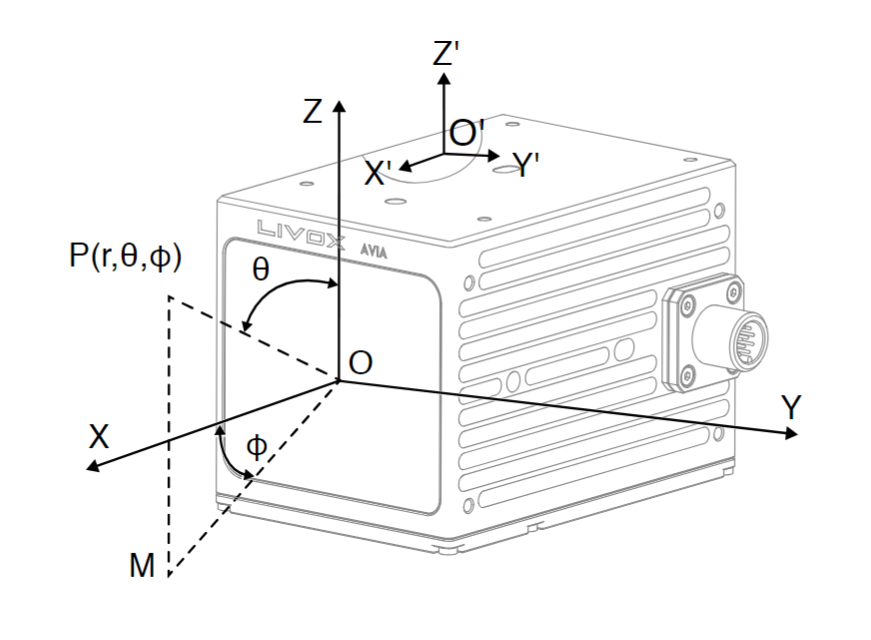
\includegraphics[width=0.8\textwidth]{figs/ch5/avia_axes.png}
    \caption{\textbf{Avia Coordinate System.}}{Taken from \textcite{AviaLiDARSensor}.}
    \label{fig:avia_axes}
\end{figure}
%----------------------------------------------------

%====================================================
\section{Data Pre-Processing}
\label{sec:ch5.section1}
%----------------------------------------------------

Before any point cloud processing can take place, the raw Avia data must be pre-processed to ensure it is in a suitable format and condition before being fed into the main processing pipeline. This pre-processing varies depending on the source of the data, but generally involves synchronising and aligning the Avia data with any ground truth data, as well as cropping and filtering the data to focus on the areas of interest and remove unwanted points produced during experimental setup.

%----------------------------------------------------
\subsection{Stationary Characterisation Data}
\label{subsec:ch5.section1.subsec1}

For the data collected during the stationary characterisation experiments, a minimal amount of pre-processing was required. The Avia was stationary during data collection, so no motion compensation was necessary. The point cloud data was rotated around the sensor's x-axis to align the data with the world frame, as the sensor was mounted at an angle of declination of approximately 16° to the horizontal during data collection. For this dataset there were no additional sensors, so no time synchronisation was required. Finally, the point cloud frames were cropped to focus on the region containing the targets, with dimensions of 3 m (length) x 2 m (width).

%----------------------------------------------------
\subsection{Simulated Motion Data}
\label{subsec:ch5.section1.subsec2}

The simulated motion data collected using the Stewart platform and motion capture system required more extensive pre-processing to ensure the Avia point cloud data was aligned and synchronised with the motion capture ground truth data. During both tests, the Stewart platform was not aligned perfectly with the motion capture system's world frame. As the Avia and motion capture system were operated independently, there was no time synchronisation between the two systems. To align the two datasets, an offset was applied to the Avia timestamps to align the start of the motion capture data with the start of the Avia data. The offsets were determined manually by inspecting the data, and identifying the point at which motion began in both datasets. For the first test (10° sweeps) the offset was determined to be -938.01 seconds, and for the second test (5° sweeps) the offset was determined to -2068.20 seconds.

During the tests, the Stewart platform was rotated around the vertical axis (Avia z-axis) relative to the motion capture system. As this test was focused on attitude estimation and was not concerned with translational motion, the Stewart platform's offset from the motion capture system's origin was inconsequential. This misalignment was corrected by applying an Euler angle rotation to the motion capture data to align it with the Avia's \ac{IMU} data. The rotation angles were determined by manually inspecting the motion capture data, and identifying the angle of rotation required to minimize the off-axis motion (motion in the roll axis when the Stewart platform was pitching and vice versa). This process was carried out for both tests, and for the first test (10° sweeps) the rotation was determined to be -42° and for the second test (5° sweeps) the rotation was determined to be -39°.

For this experiment, the point cloud data was not used and thus no pre-processing was required.

%----------------------------------------------------
\subsection{Aalto Data}
\label{subsec:ch5.section1.subsec3}

The data collected from the Aalto University wave and ice tank was the only point cloud data used in this investigation that was not collected using \ac{ROS}. The data was instead collected using the Livox SDK, which stores the point cloud data in the proprietary Livox \emph{.lvx} format. Livox provides tools to convert \emph{.lvx} files into \emph{.bag} files (\cite{livoxLivoxSDKLivox_ros_driver2025}), allowing the data to be processed using the same tools developed for the other datasets. Once the point cloud data was imported into MATLAB, it was rotated about the sensor's x-axis, similarly to the stationary characterisation data, as the sensor was mounted at an angle of declination of approximately 30° to the horizontal during data collection. Next, the point cloud data was cropped to remove unwanted points created during experimental setup, such as those from the tank walls and wave makers.

At the beginning of each test, there was a period of time when the waves were still settling into their steady state, and had not yet reached the set amplitude and frequency. To ensure that only steady state wave data was processed, both the point cloud data and wave probe data were trimmed to exclude this initial settling period.

The wave probe and Avia were not time synchronised during this experiment and due to the nature of the experimental setup and data collected, it was not possible to synchronise the data from the two sensors.

%----------------------------------------------------
\subsection{SCALE Data}
\label{subsec:ch5.section1.subsec4}

Almost all the data collected during the \ac{SCALE} Winter 2022 Cruise required no pre-processing before being fed into the main processing pipeline. There were no additional sensors used during data collection, so no time synchronisation was required. Minimal unwanted points were created during experimental setup, so no cropping was necessary. The noise and motion artefacts present in the data were dealt with during the main processing pipeline, thus the only pre-processing required was to trim the data to only include the periods when the Avia was actively collecting data and exclude idle and setup periods.

%====================================================
\section{Sensor Characterisation}
\label{sec:ch5.section2}
%----------------------------------------------------

Before analysing the outputs of the main processing pipeline, it is important to understand the characteristics and limitations of the Livox Avia sensor. This section details the investigations carried out to determine the strengths and weaknesses of the Avia in the context of observing sea ice in the \ac{MIZ} from a moving platform.

The Avia was designed primarily for use in urban environments for mapping, navigation and surveying applications (\cite{AviaLiDARSensor}). This means that the sensor has been optimised for capturing static scenes from a stable observation platform, aimed perpendicular to the target scene. This is almost the exact opposite of the observation conditions in the \ac{MIZ}, where the target scene (sea ice field) is highly dynamic, the observation platform is never fully stable, and the sensor is mounted at an angle to the target scene. Therefore, it is important to understand how these differences in observation conditions affect the quality of the captured data.

The primary areas of investigation were the accuracy of the captured scene when the sensor is not perpendicular to the target scene, leading to shadowing and decreased point density, the minimum number of frames required to obtain accurate recreations of the target scene and the impact of the sensor's beam divergence. The outcomes of these investigations informed the final design of the data processing pipeline.

%----------------------------------------------------
\subsection{Target Scene Reconstruction}
\label{subsec:ch5.section2.subsec1}

To evaluate the Avia's ability to accurately reconstruct a target scene, the data collected during the stationary characterisation experiments was analysed. The point cloud data collected from the four board configurations were compared to the known geometry of the boards to determine the accuracy of the reconstructed scene and identify the impact of the sensor's angle of incidence, shadowing effects, beam divergence, and point density on the quality of the reconstructed scene.

This was achieved by comparing a single frame of point cloud data to the known geometry of the boards, and any deviations from the expected geometry were noted. Consecutive frames were then concatenated to the initial frame, and the reconstruction quality was re-evaluated. This process was repeated, with no more than 15 frames (corresponding to 1.5 seconds) being concatenated at a time. This process was applied to all four board configurations, and the minimum number of frames required to achieve an accurate reconstruction of the target scene noted.

%----------------------------------------------------
\subsection{Target Normals Estimation}
\label{subsec:ch5.section2.subsec2}

To further evaluate whether valuable information about the target scene can be extracted from the Avia point cloud data, the quality of estimated point normals was investigated. MATLAB's \emph{pcnormals} function was used to estimate the point normals from the final concatenated point clouds created during the target scene reconstruction investigation. The \emph{pcnormals} function estimates point normals by fitting a plane to the \emph{k} nearest neighbours of each point in the point cloud, and using the normal vector of the fitted plane as the estimated normal vector for the point (\cite{PcnormalsEstimateNormals}). \emph{k} was set to 5 for this investigation, as it is expected that there will be a low density of points in the final point cloud frame, and a small \emph{k} value will allow for more accurate normal estimations, while a larger \emph{k} value may lead to over-smoothing of the normals.

The estimated normals are compared to the known geometry of the boards and to the reconstructed scene to determine their accuracy and usefulness in inferring target geometry.

%====================================================
\section{Summary}
\label{sec:ch5.section3}
%----------------------------------------------------

This chapter detailed the pre-processing steps taken to prepare the collected data for analysis and further processing, as well as the methods used to characterise the performance and behaviour of the Avia sensor. The pre-processing steps varied depending on the source of the data, but generally involved synchronising and aligning the Avia data with any ground truth data, as well as cropping the data to focus on the areas of interest. The sensor characterisation investigations focused on evaluating the Avia's ability to accurately reconstruct a target scene and estimate point normals, which will inform the design of the final data processing pipeline and the interpretation of the results obtained from the pipeline.

%****************************************************
% END
%****************************************************